% -*- coding: utf-8 -*-
% !TeX program = xelatex
\documentclass[UTF8,a4paper,10pt]{ctexart}

% 保留课程模板的版心、封面和页眉页脚风格。
\usepackage[left=3.17cm,right=3.17cm,top=2.74cm,bottom=2.74cm]{geometry}
\usepackage{amsmath,amssymb}
\usepackage{graphicx}
\usepackage{float}
\usepackage{booktabs}
\usepackage{multirow}
\usepackage{array}
\usepackage{tabularx}
\usepackage{xcolor}
\usepackage{listings}
\usepackage{enumitem}
\usepackage{fancyhdr}
\usepackage{cite}
\usepackage[colorlinks=true,linkcolor=black,citecolor=black,urlcolor=blue]{hyperref}

\ctexset{
  section={name={,、},number=\chinese{section},format=\Large\bfseries},
  subsection={name={（,）},number=\chinese{subsection},format=\large\bfseries},
  subsubsection={name={,.},number=\arabic{subsubsection},format=\normalsize\bfseries}
}

\pagestyle{fancy}
\fancyhf{}
\lhead{\kaishu 自然语言处理第一次作业}
\rhead{\kaishu 实验报告}
\cfoot{\thepage}
\renewcommand{\headrulewidth}{0.1pt}
\renewcommand{\footrulewidth}{0pt}
\newcommand{\HRule}{\rule{\linewidth}{0.5mm}}

\setlength{\parindent}{2em}
\setlength{\parskip}{0.25em}
\renewcommand{\arraystretch}{1.18}
\linespread{1.20}

\lstset{
  language=Python,
  basicstyle=\ttfamily\small,
  keywordstyle=\color{blue!70!black}\bfseries,
  commentstyle=\color{green!45!black},
  stringstyle=\color{orange!55!black},
  numbers=left,
  numberstyle=\tiny\color{gray},
  frame=single,
  breaklines=true,
  showstringspaces=false
}

\newcommand{\method}[1]{\texttt{#1}}

\begin{document}

\begin{titlepage}
  \begin{center}
    
\includegraphics[width=0.8\textwidth]{NKU.png}\\[1cm]
    {\Huge \kaishu 南\ \ \ \ \ 开\ \ \ \ \ 大\ \ \ \ \ 学}\\[0.9cm]
    {\huge \kaishu 计\ \ 算\ \ 机\ \ 学\ \ 院}\\[0.5cm]
    {\Large \bfseries 实验报告}\\[0.8cm]
    \HRule\\[0.9cm]
    {\LARGE\bfseries 作业一：文本分类实现}\\[0.4cm]
    {\large Bag of Words、Word Embedding 与 BERT}
    \\[0.7cm]
    \HRule\\[1.7cm]
    {\LARGE \kaishu 姓名\ :\ \underline{\makebox[5cm][c]{程子晨}}}\\[0.5cm]
    {\LARGE \kaishu 学号\ :\ \underline{\makebox[5cm][c]{2312390}}}\\[0.5cm]
    {\LARGE \kaishu 专业\ :\ \underline{\makebox[5cm][c]{计算机科学与技术}}}\\[0.5cm]
    \vfill
    {\Large 2026 年 10 月}
  \end{center}
\end{titlepage}

\begin{abstract}
本报告在统一的 NYT 新闻三分类数据划分上，对二值词袋、词频词袋、预训练 GloVe、两种语料训练的 Word2Vec 和 BERT 微调进行比较。六组实验均按课程要求在同一测试集上报告 Accuracy 与 Macro-F1。词频词袋加 Logistic Regression 取得最高的 0.9913 Accuracy 和 0.9789 Macro-F1。进一步复算逐类指标发现，最佳模型的 10 个错误中有 8 个发生在 business 与 politics 之间；对原始数据的审计还发现 10 篇测试正文与训练集完全重复。剔除这些重叠测试样本后，词频模型的 Accuracy 和 Macro-F1 分别为 0.9912 和 0.9785。此外，全部测试新闻的 BERT 输入长度均超过作业规定的 64 token 上限。上述补充分析帮助区分真实观测、潜在数据泄漏和模型结构带来的解释限制。
\end{abstract}
\noindent\textbf{关键词：}文本分类；词袋模型；词向量；BERT；Macro-F1；数据泄漏

\section{实验目的}

本实验以 New York Times（NYT）新闻三分类为统一任务，比较不同文本表示方法在相同数据划分、相同评价指标下的实际效果。实验依次实现二值词袋、词频词袋、预训练 GloVe、分别在 AG News 与 NYT 训练集上训练的 Word2Vec，以及 BERT-base-uncased 微调，共六组模型。除 BERT 外，其余模型均使用 Logistic Regression 完成分类。

实验重点包括：理解稀疏词袋表示与稠密词向量表示的差异；掌握对词向量求平均得到文档表示的方法；完成预训练语言模型的端到端微调；使用 Accuracy 与 Macro-F1 评价类别不均衡条件下的分类效果；保证全部方法共享同一份 NYT 训练集、验证集和测试集，使结果具有可比性。

围绕统一任务，报告重点回答三个问题：保留词频是否优于只记录词是否出现；不同来源的 100 维词向量在相同分类器下有何差异；在 64 token 截断约束下，BERT 微调结果应如何与处理全文的传统方法比较。所有结论均限定于本次数据划分和已运行的配置，不将相关性解释为已验证的因果关系。

\section{实验原理}

\subsection{数据集与统一划分}

NYT 数据包含新闻正文 \method{text} 与类别 \method{label} 两列，共 11,519 条有效样本，类别为 business、politics 和 sports。代码首先检查必需列、剔除缺失或空正文，再通过两次分层随机划分，按 80\%/10\%/10\% 生成训练集、验证集和测试集；随机种子固定为 42。分任务运行时，程序用相同的数据文件和种子重新生成划分，并将各子集保存为 CSV；输出目录还记录原始文件的 SHA-256，防止混用不同数据或随机种子的结果。最终指标只在 NYT Test Set 上计算。

\begin{table}[H]
  \centering
  \caption{NYT 数据集划分与类别分布}
  \label{tab:split}
  \begin{tabular}{lrrrrr}
    \toprule
    数据子集 & 比例 & business & politics & sports & 合计 \\
    \midrule
    Training Set   & 80\% & 1,143 & 1,161 & 6,911 & 9,215 \\
    Validation Set & 10\% &   143 &   145 &   864 & 1,152 \\
    Test Set       & 10\% &   143 &   145 &   864 & 1,152 \\
    \midrule
    全部            & 100\% & 1,429 & 1,451 & 8,639 & 11,519 \\
    \bottomrule
  \end{tabular}
\end{table}

用于训练词向量的 AG News 数据由 90,000 条新闻文本组成，只用于 Task 2 中的 AG News Word2Vec，不参与 NYT 分类器的数据划分。NYT 原始类别分布明显不均衡：sports 为 8,639 条，约占 75.0\%；business 和 politics 分别为 1,429 与 1,451 条。因此除了 Accuracy，还必须关注 Macro-F1。

词袋和词向量方法采用同一套轻量英文分词规则：先转小写，再用正则表达式提取英文单词、带撇号的英文词和数字；词袋特征和词向量查找均沿用这一规则。BERT 使用其预训练模型自带的 WordPiece tokenizer，不能与前述词级分词完全等同。

\subsection{Task 1：Bag of Words}

设训练语料建立的词表为 $V$，一篇文档为 $d$。二值词袋只记录词是否出现：
\begin{equation}
  x_i=\begin{cases}
  1, & w_i\in d,\\
  0, & w_i\notin d.
  \end{cases}
\end{equation}
词频表示则记录单词在当前文档中的出现次数：
\begin{equation}
  x_i=\operatorname{count}(w_i,d),\qquad \mathbf{x}\in\mathbb{R}^{|V|}.
\end{equation}

代码使用 \method{CountVectorizer} 在 Training Set 上拟合词表，再分别设置 \method{binary=True} 与 \method{binary=False}。两种表示得到的词表大小均为 65,608。分类器为多类别 Logistic Regression，正则化参数 $C=1.0$，优化器为 L-BFGS，最大迭代次数为 2,000。测试集只调用训练阶段已拟合的向量器进行变换，不参与词表构建。

若类别数为 $K$，分类器从文档特征 $\mathbf{x}$ 计算各类得分 $\mathbf{w}_k^\top\mathbf{x}+b_k$，经 softmax 得到类别概率，最后取最大概率对应的类别。该模型直接利用词项特征或 100 维文档向量完成分类；词袋矩阵保持稀疏存储，避免将 65,608 维特征扩展为稠密矩阵。

\subsection{Task 2：Word Embedding 与 Word2Vec}

三组词向量实验均使用 100 维单词向量。对于分词后的文档 $d=(w_1,\ldots,w_n)$，只对能够在词向量表中找到的 $m$ 个有效单词取平均：
\begin{equation}
  \mathbf{e}(d)=\frac{1}{m}\sum_{i=1}^{m}\mathbf{e}(w_i),
  \qquad \mathbf{e}(d)\in\mathbb{R}^{100}.
\end{equation}
若文档中没有任何已知词，则使用 100 维零向量；实际运行中三种方法的零向量文档数均为 0。得到文档向量后，仍采用与 Task 1 相同配置的 Logistic Regression。

\begin{enumerate}[leftmargin=2.3em]
  \item \textbf{Pre-trained GloVe：}实际实验使用 Gensim 发布的 Wiki 2014 + Gigaword 5（6B tokens）100 维 GloVe 词向量\cite{pennington2014}\footnote{Gensim 模型标识为 \texttt{glove-wiki-gigaword-100}；其元数据说明该模型由 Stanford GloVe 6B 词向量转换格式而来。}。这与作业指定的 \method{glove.6B}、100 维配置一致。完整词表包含 400,000 个词；代码只保留 NYT 文本实际需要的词向量。
  \item \textbf{Word2Vec Trained on AG News：}在 90,000 条 AG News 文本上自行训练 Skip-gram Word2Vec\cite{mikolov2013}。
  \item \textbf{Word2Vec Trained on NYT：}只使用 NYT Training Set 训练 Word2Vec，避免 Validation Set 与 Test Set 的信息泄漏。
\end{enumerate}

两组自行训练的 Word2Vec 均设置向量维数为 100、窗口大小为 5、\method{min\_count=2}、Skip-gram（\method{sg=1}）、训练 10 个 epoch。为降低多线程训练与 Python 哈希随机化造成的差异，实验使用单 worker 和固定的稳定哈希函数。

\subsection{Task 3：BERT 微调}

BERT 实验严格使用 \method{google-bert/bert-base-uncased}\cite{devlin2019}。Tokenizer 将每篇新闻截断至最大 64 个 token，短序列在 batch 内动态补齐。分类头输出三个类别的 logits，并通过交叉熵损失进行端到端训练。训练轮数为 3，batch size 为 16，学习率为 $2\times10^{-5}$，weight decay 为 0.01。

每个 epoch 结束后在 Validation Set 上计算 Macro-F1 并保存检查点，训练结束时自动恢复验证集 Macro-F1 最高的检查点，再在 Test Set 上进行一次最终评价。三轮训练都已完成；最佳检查点的选择只依赖验证集，不依据测试集表现调整参数。

\subsection{评价指标}

设测试集样本数为 $N$，预测正确的样本数为 $N_{\mathrm{correct}}$，则
\begin{equation}
  \mathrm{Accuracy}=\frac{N_{\mathrm{correct}}}{N}.
\end{equation}
对类别 $k$，先计算 Precision 与 Recall，再得到
\begin{equation}
  F1_k=\frac{2P_kR_k}{P_k+R_k},\qquad
  \mathrm{Macro\mbox{-}F1}=\frac{1}{K}\sum_{k=1}^{K}F1_k.
\end{equation}
本数据集中 sports 占比约 75\%，因此 Accuracy 容易受到多数类影响；Macro-F1 对三个类别等权平均，可更直接地反映少数类上的分类能力。

为说明两个指标的差别，可以构造无需训练的“恒预测 sports”参照：它在测试集上可答对 $864/1152=0.7500$ 的样本，但 business 与 politics 的 F1 均为 0，sports 的 F1 为 $2\times0.75/(1+0.75)=0.8571$，因此 Macro-F1 只有 0.2857。该数值是依据测试集类别数量计算的理论参照，不计入六组规定实验，也未用测试标签训练模型。

\subsection{代码实现与运行环境}

实验入口为 \path{run.py}。\path{nlp_assignment/data.py} 负责加载和划分数据；\path{bow.py} 构建两种词袋特征；\path{embeddings.py} 负责 GloVe 读取、Word2Vec 训练和平均池化；\path{bert.py} 实现预训练模型微调；\path{common.py} 统一标签编码、逻辑回归、指标计算和结果保存。不同实验均调用同一个指标函数，结果写入 \path{outputs/results.json} 与 \path{outputs/results.csv}。实验在 Windows、Python 3.12 环境中运行；BERT 使用 NVIDIA GeForce RTX 4060 Laptop GPU 与 CUDA 12.4 版本的 PyTorch，传统模型使用 scikit-learn 与 Gensim。

词袋与平均词向量的逻辑回归直接在 Training Set 上拟合；Validation Set 主要用于 BERT 的模型选择。代码没有使用验证集反复调节逻辑回归超参数，因此其测试结果对应事先固定的默认配置，而不是经过搜索得到的最优分数。这一点有利于比较各类文本表示，但也限定了结果解释范围。

\section{实验结果分析}

\subsection{总体结果}
\enlargethispage{2\baselineskip}

表~\ref{tab:results} 汇总六种方法在同一 NYT Test Set（1,152 条样本）上的真实运行结果。Word Frequency 在两个指标上均取得最高值，Accuracy 为 0.9913，Macro-F1 为 0.9789；Binary Bag of Words 次之。所有方法的 Accuracy 均超过 0.975，说明新闻类别在词汇层面具有较强的可分性。

为便于核对 Accuracy，测试集上的正确分类数分别为：二值词袋 1,139 条、词频词袋 1,142 条、GloVe 与 NYT Word2Vec 各 1,135 条、AG News Word2Vec 1,124 条、BERT 1,131 条。这些整数除以 1,152 后与表中 Accuracy 一致。表中指标保留四位小数，完整精度保存在 JSON 结果文件中。

\begin{table}[H]
  \centering
  \caption{六种文本分类方法在 NYT Test Set 上的结果}
  \label{tab:results}
  \begin{tabularx}{\textwidth}{>{\raggedright\arraybackslash}Xcc}
    \toprule
    方法 & Accuracy & Macro-F1 \\
    \midrule
    Binary Bag of Words + LR            & 0.9887 & 0.9718 \\
    \textbf{Word Frequency + LR}         & \textbf{0.9913} & \textbf{0.9789} \\
    Pre-trained GloVe 100d + LR          & 0.9852 & 0.9646 \\
    AG News Word2Vec 100d + LR           & 0.9757 & 0.9403 \\
    NYT Training Set Word2Vec 100d + LR  & 0.9852 & 0.9635 \\
    BERT-base-uncased                    & 0.9818 & 0.9601 \\
    \bottomrule
  \end{tabularx}
\end{table}

\begin{figure}[H]
  \centering
  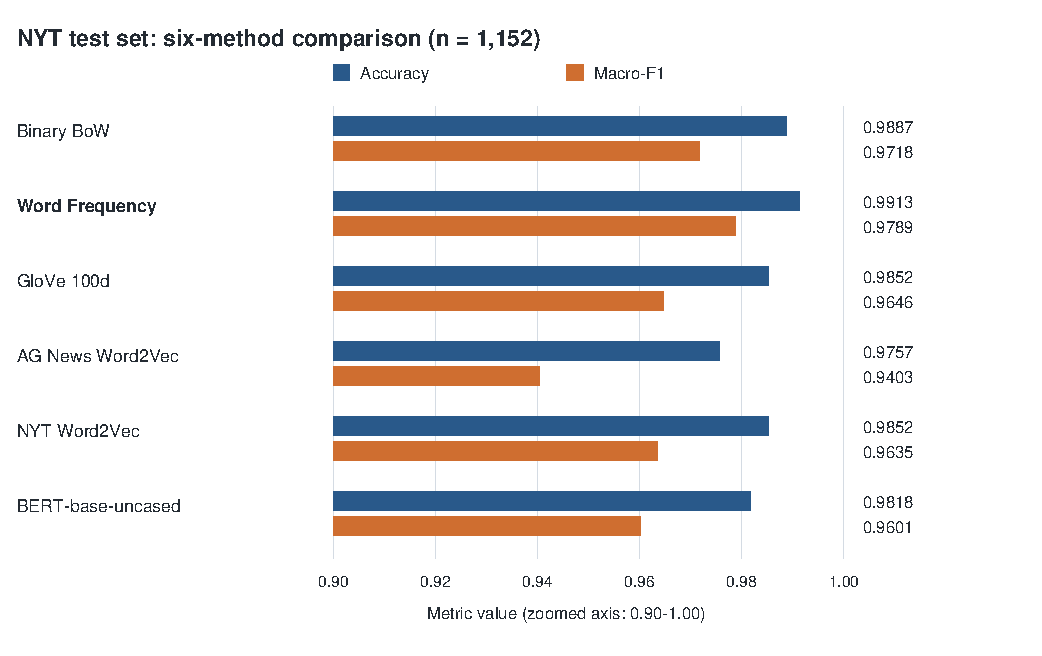
\includegraphics[width=0.98\textwidth]{figures/overall_metrics.pdf}
  \caption{六种方法在同一 NYT 测试集上的指标对比。横轴从 0.90 而非 0 开始，以便展示高分区间的细小差异；精确比较应以表~\ref{tab:results} 中的数值为准。}
  \label{fig:overall}
\end{figure}

\subsection{横向比较与指标差距}

由图~\ref{fig:overall} 可见，两种词袋方法在 Accuracy 和 Macro-F1 上均占前两位；预训练 GloVe 与 NYT Word2Vec 的 Accuracy 并列第三；BERT 位于其后，AG News Word2Vec 最低。若仅看 Accuracy，六组方法都超过 0.975，似乎差别不大；但结合 Macro-F1，AG News Word2Vec 与最高的词频词袋相差约 3.85 个百分点，这比二者约 1.56 个百分点的 Accuracy 差距更明显。两项指标共同表明：在本次不均衡的三分类数据上，高总体正确率并不能替代对各类平衡表现的检查。

把准确率转换为同一测试集上的错误篇数，可得到词频词袋 10 篇、二值词袋 13 篇、GloVe 和 NYT Word2Vec 各 17 篇、BERT 21 篇、AG News Word2Vec 28 篇。词频词袋相对二值词袋少错 3 篇，相对 BERT 少错 11 篇；由于测试集只有 1,152 篇，表中看似微小的千分位差异对应的是有限数量的样本。各方法的 Macro-F1 排序与 Accuracy 排序总体一致，但不能仅凭一次划分与这些差值推断统计显著性。

\begin{samepage}
从表示与输入范围看，词袋方法在 65,608 维稀疏空间保留具体词项，平均词向量方法把全文压缩到 100 维，BERT 则对前 64 token 构建上下文表示并端到端训练。前五组方法都使用同配置的 Logistic Regression，而 BERT 使用自己的分类头；因此图~\ref{fig:overall} 比较的是\emph{完整实验流水线}的结果，不是只改变表示而其他条件完全不变的严格消融实验。坐标轴为放大刻度，图形长度不应被解释为从零开始的比例。
\end{samepage}

\subsection{词袋模型分析}

Word Frequency 相比 Binary Bag of Words 的 Accuracy 提高约 0.26 个百分点，Macro-F1 提高约 0.71 个百分点。两种模型使用完全相同的词表与分类器，差异只来自特征值定义，因此结果表明词频不仅保留了关键词是否出现的信息，还提供了重复出现所反映的主题强度。对 politics、business 与 sports 这类主题分类任务，类别指示词及其出现频次通常具有直接判别力，稀疏高维表示没有因平均池化而丢失这些局部词汇线索。

从实现看，二值词袋与词频词袋均对训练集拟合词表，再对测试集做变换；词频方法没有使用 TF-IDF、归一化或额外的类别特征。因此本组比较主要反映「是否保留词项出现次数」的作用。不过只进行了一次固定划分，约 0.26 个百分点的差距对应 3 篇测试文章，不能据此断言该差距在其他随机划分上稳定成立。

\subsection{词向量模型分析}

GloVe 与 NYT Word2Vec 的 Accuracy 相同，均为 0.9852，Macro-F1 分别为 0.9646 和 0.9635。两者差距很小，说明通用预训练词向量与域内训练词向量在本实验的平均池化框架下取得了相近效果。NYT Word2Vec 的测试 token 覆盖率最高，但覆盖率提升并未直接转化为更高的 Macro-F1，表明覆盖率不是性能的唯一决定因素；词向量质量、训练语料规模以及平均池化造成的词序丢失同样重要。

与词频词袋相比，GloVe 的 Accuracy 低约 0.61 个百分点、Macro-F1 低约 1.43 个百分点，测试集多错 7 篇。两者共用 Logistic Regression，却把文档从 65,608 维稀疏词项特征变为 100 维平均词向量；这种压缩有利于使用稠密特征，但精确的主题词身份和词序等信息不再被直接保留。本实验不能单独分离维度压缩、预训练语料与词向量质量各自的作用，因此不把这 7 篇差异归因于其中任何单一因素。

\begin{table}[H]
  \centering
  \caption{词向量覆盖率与词表规模}
  \label{tab:coverage}
  \begin{tabular}{lccc}
    \toprule
    词向量来源 & Training token 覆盖率 & Test token 覆盖率 & 词表规模 \\
    \midrule
    GloVe 6B 100d       & 98.18\% & 98.16\% & --- \\
    AG News Word2Vec    & 97.11\% & 97.11\% & 37,589 \\
    NYT Train Word2Vec  & 99.68\% & 99.21\% & 46,085 \\
    \bottomrule
  \end{tabular}
\end{table}

AG News Word2Vec 的 Accuracy 和 Macro-F1 均为三种词向量方法中最低。其训练语料与 NYT 分类任务存在来源和主题分布差异，且测试 token 覆盖率也最低，这与结果下降的方向一致。不过，本实验没有单独控制语料规模、词频分布和领域差异，因此不能把性能差异完全归因于某一个因素。

按 770,680 个测试词级 token 计数，GloVe、AG News Word2Vec、NYT Word2Vec 分别有 14,164、22,310、6,055 个 token 无法在对应词向量表中查到；但三种方法均不存在“整篇文章没有任何可用词向量”的零向量样本。因此 AG News 的劣势不能简单解释成大量文档完全无法表示。NYT 的覆盖率最高却未超过 GloVe，也进一步表明\emph{覆盖多少词}与\emph{已覆盖词向量能否有效区分类别}是不同问题。上述覆盖率按 token 频次计算，不等于词表类型覆盖率。

两组自行训练的 Word2Vec 使用同样的 100 维、Skip-gram、窗口 5 和 10 epoch 设置。NYT Word2Vec 比 AG News Word2Vec 的 Accuracy 高约 0.95 个百分点、Macro-F1 高约 2.31 个百分点，对应少错 11 篇。值得注意的是，AG News 训练文本有 90,000 篇，而 NYT 训练集仅有 9,215 篇；更多训练文章并未在本次迁移分类任务中带来更好结果。但两语料的平均长度、词汇分布、类别主题和数据来源都不同，\emph{不能}从这一对结果推出“训练语料越少越好”或领域匹配是唯一原因。GloVe 与 NYT Word2Vec 各错 17 篇，Macro-F1 只相差约 0.11 个百分点，也不宜据此作强排序。

平均池化还有一项共同限制：词向量的求和交换顺序不改变结果，模型无法直接表示词序、否定范围或关键词在文中的位置。同一个词重复出现会在均值中产生更大权重，但长文中的少数强判别词也可能被大量一般词汇稀释。这些是模型结构上的限制，并非本实验已单独测量的错误来源。

\subsection{BERT 结果分析}

BERT 的 Accuracy 为 0.9818，Macro-F1 为 0.9601，未超过两种词袋模型。该结果不应外推为预训练模型普遍弱于词袋模型。对保存的 NYT Test Set 使用最终 BERT tokenizer 统计，1,152 篇新闻在未截断时的序列长度全部超过 64 token，中位数约为 889 token；按作业要求设定 \method{max\_length=64} 后，所有测试新闻都只保留前 64 个 token，样本保留比例的中位数约为 7.2\%。词袋与平均词向量方法则处理全文，因此三类表示实际利用的文本范围不同，BERT 指标应在这一约束下理解。

长度分布并非只由极少数超长文章造成：未截断序列的第 25 与第 75 百分位分别约为 605 和 1,078 token，最短一篇也有 75 token。这意味着 64 token 上限影响每一篇测试文章，而不是偶发边界情况；不过这些长度统计本身仍无法测出截断对某个类别或某种错误的因果影响。

此外，BERT 仅训练 3 个 epoch，学习率和 batch size 也没有做系统搜索。它在本次设置下优于 AG News Word2Vec 的 Macro-F1，但比 GloVe 与 NYT Word2Vec 略低。截断、训练设置与模型结构可能共同影响结果；本实验没有进行更长序列的对照实验，不能量化截断本身造成了多少性能差异。

若以错误篇数比较，BERT 的 21 篇介于 GloVe/NYT Word2Vec 的 17 篇与 AG News Word2Vec 的 28 篇之间；其 Macro-F1 比 AG News Word2Vec 高约 1.98 个百分点，却比最佳词频词袋低约 1.87 个百分点。BERT 能建模上下文和词序，平均词向量与词袋则分别牺牲词序或上下文交互；然而在本实验中，BERT 的输入仅保留每篇新闻开头约 7.2\% 的 token（保留比例中位数），而其余方法读取全文。这使得“更强的表示机制”与“更少的可见文本”同时存在，不能仅根据分数判断哪类表示在等量输入下更优。

六种方法的 Macro-F1 均低于 Accuracy，差距在 AG News Word2Vec 上最明显。这与表~\ref{tab:split} 所示的类别不均衡相符：多数类 sports 对 Accuracy 的贡献较大，而 Macro-F1 会等权计入 business 与 politics。因而本实验不能只依据 Accuracy 排序，Macro-F1 是判断少数类分类质量不可缺少的指标。

原始结果文件仅保存各方法的总体 Accuracy 与 Macro-F1，并未保存逐类别 F1 或混淆矩阵。因此，单靠表~\ref{tab:results} 不能断定 business 和 politics 哪类更难识别；下文利用已保存的训练划分和模型文件重建六组预测，以便补充这一层面的分析。六组复算指标均与原始记录吻合。

\subsection{六种方法的逐类别能力}

图~\ref{fig:all-class-f1} 将六组方法的三个类别 F1 放在同一尺度下比较。所有方法的 sports F1 均高于 0.994，而 business 和 politics 的 F1 变化更大：business 从 AG News Word2Vec 的 0.9072 到词频词袋的 0.9658，跨度约 5.85 个百分点；politics 对应从 0.9167 到 0.9720，跨度约 5.54 个百分点。相比之下，sports 的最大跨度不足 0.41 个百分点。由此可见，整体 Macro-F1 的差异主要反映两个少数类的识别能力，而不是 sports 的细小波动。

\begin{figure}[H]
  \centering
  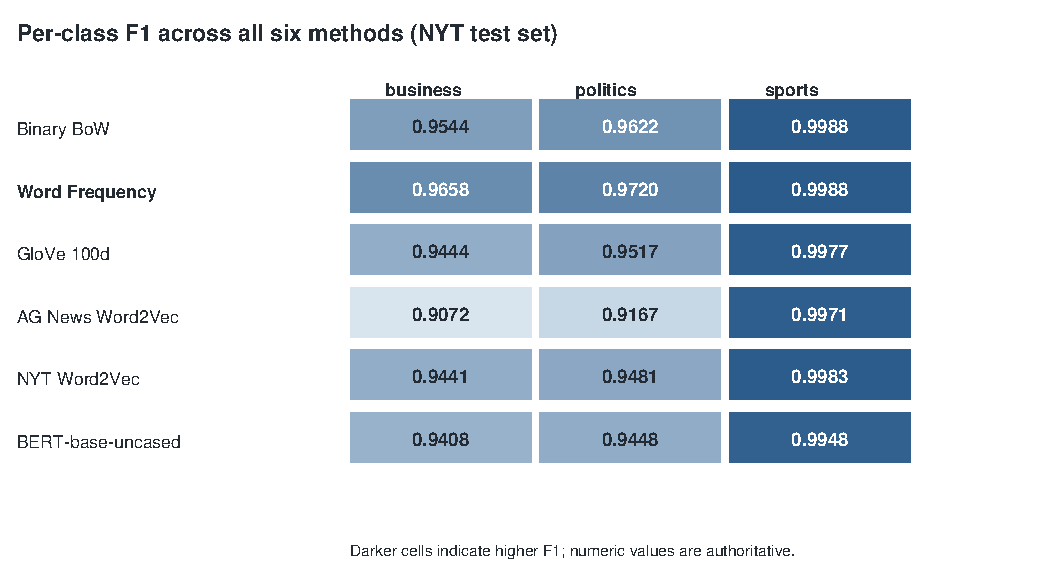
\includegraphics[width=0.96\textwidth]{figures/all_class_f1.pdf}
  \caption{六种方法的逐类别 F1 热力图。每格给出实际 F1 数值；色阶只用于辅助比较，不代表类别样本量。三类测试样本数分别为 143、145、864。}
  \label{fig:all-class-f1}
\end{figure}

从召回率进一步观察，词频词袋在 business 上达到 0.9860，为六组最高；但其 politics 召回率 0.9586 略低于二值词袋的 0.9655。也就是说，词频信息提高了整体少数类 F1，却并非对每一类、每一项指标都单调改善。AG News Word2Vec 的 business 和 politics 召回率分别仅为 0.9231 和 0.9103，对应图中两类的最低 F1。BERT 的 sports F1 为 0.9948，虽仍然很高，却是六组中最低的 sports F1；不能仅用“BERT 在少数类吃亏”概括其错误分布。

\subsection{逐类误差与词汇判别线索}

为补充总体指标，按原代码的分词、\method{CountVectorizer(binary=False)} 和 Logistic Regression 配置，在保存的 Training Set 上重新拟合词频模型，并对同一 Test Set 预测。复算所得 Accuracy 为 0.991319、Macro-F1 为 0.978874，与原结果文件完全一致。表~\ref{tab:class-metrics} 和表~\ref{tab:confusion} 给出这一\emph{最佳词频模型}的逐类指标及混淆矩阵；行是真实类别，列是预测类别。

\begin{table}[H]
  \centering
  \caption{词频词袋模型的逐类别测试结果}
  \label{tab:class-metrics}
  \begin{tabular}{lrrrr}
    \toprule
    类别 & 样本数 & Precision & Recall & F1 \\
    \midrule
    business & 143 & 0.9463 & 0.9860 & 0.9658 \\
    politics & 145 & 0.9858 & 0.9586 & 0.9720 \\
    sports   & 864 & 1.0000 & 0.9977 & 0.9988 \\
    \bottomrule
  \end{tabular}
\end{table}

\begin{figure}[H]
  \centering
  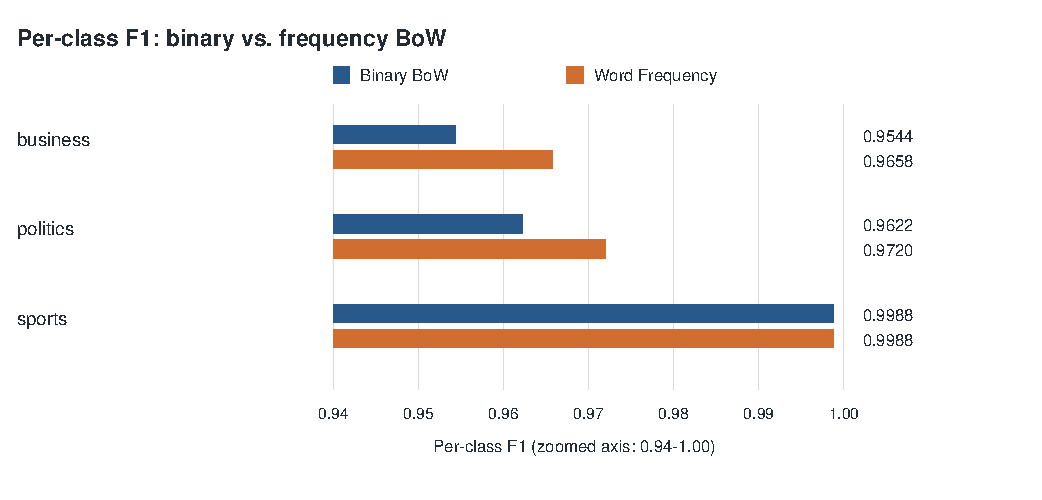
\includegraphics[width=0.98\textwidth]{figures/bow_class_f1.pdf}
  \caption{二值词袋与词频词袋的逐类 F1。横轴从 0.94 开始，是用于展示细微差别的放大刻度；两模型的逐类指标由保存划分重新拟合得到。}
  \label{fig:class-f1}
\end{figure}

\begin{table}[H]
  \centering
  \caption{词频词袋模型的测试集混淆矩阵}
  \label{tab:confusion}
  \begin{tabular}{lrrr}
    \toprule
    真实类别 $\backslash$ 预测类别 & business & politics & sports \\
    \midrule
    business & 141 & 2 & 0 \\
    politics & 6 & 139 & 0 \\
    sports   & 2 & 0 & 862 \\
    \bottomrule
  \end{tabular}
\end{table}

矩阵中 10 个错误有 8 个发生在 business 与 politics 之间；sports 几乎全部识别正确。如图~\ref{fig:class-f1} 所示，与二值词袋相比，词频模型的 business F1 从 0.9544 提高至 0.9658，politics 的 F1 从 0.9622 提高至 0.9720，而 sports 的 F1 四舍五入后均为 0.9988。因此总体 Macro-F1 的改善主要来自两个少数类，而非占 75\% 的 sports；但仍有 6 篇 politics 被误判为 business。逐类分析比单看总体准确率更能指出后续改进方向。

检查词频模型的正向系数，sports 类中权重靠前的词包括 \emph{game}、\emph{team}、\emph{players}；politics 类包括 \emph{washington}、\emph{law}、\emph{republican}；business 类包括 \emph{company}、\emph{flight}、\emph{oil}。这些词与新闻主题基本一致，支持词汇特征对该任务具有判别力的观察。不过，原始词频未经标准化，系数大小会受词频与特征相关性影响，不能把单个高权重词解释为因果依据。

\subsection{错误类型、共同难例与互补性}

将每个模型的非对角混淆矩阵单元分为两类：business 与 politics 之间的互相误判，以及至少涉及 sports 的误判。图~\ref{fig:error-types} 显示，前一类分别占六组总错误的 11/13、8/10、13/17、23/28、14/17 和 12/21。传统方法的主要瓶颈均是 business--politics 边界；BERT 的该类错误仍有 12 篇，但另有 9 篇涉及 sports，在六组中数量最多。因此不同方法的错误结构并不完全相同，不能只按总错误数判断潜在改进点。

\begin{figure}[H]
  \centering
  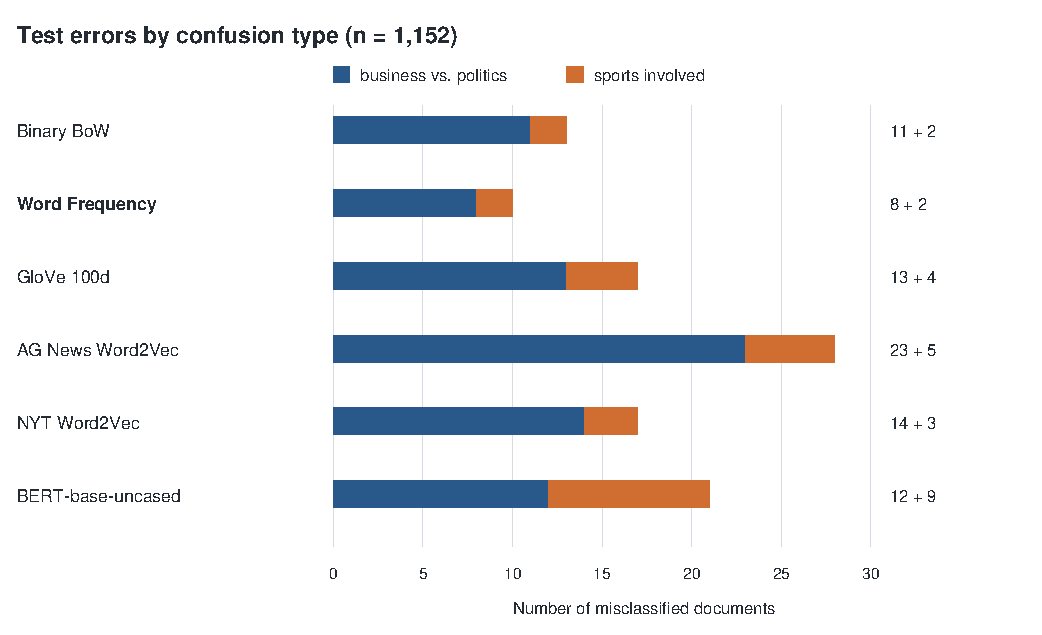
\includegraphics[width=0.96\textwidth]{figures/error_types.pdf}
  \caption{六种方法测试错误的类型分解。两段长度之和为该方法的总错误篇数；business--politics 表示两个少数类之间的双向误判，sports 相关表示任一方向涉及 sports 的误判。}
  \label{fig:error-types}
\end{figure}

把六组模型在同一测试样本上的对错逐篇对齐，1,106/1,152 篇（96.0\%）由全部方法共同判对；剩余 46 篇至少被一种方法判错，其中 23 篇只被一种方法判错，另有 3 篇被全部六组方法判错。这说明分歧集中在很小的测试子集，也提示融合模型可能只在少量边界样本上有空间；但仅凭错误重叠计数，既不能保证简单投票有收益，也不能断定那 3 篇共同难例一定存在标签问题。

\subsection{同一样本上的配对比较}

由于六种方法使用完全相同的测试文章，只比较两个总体百分数会丢失逐样本配对信息。以分数最高的词频词袋为参照，表~\ref{tab:paired} 列出两模型预测正确性不一致的篇数，并对“双方各自独有的正确篇数相同”做双侧精确 McNemar 检验。五次比较再用 Holm 方法控制多重检验的家族错误率。该检验针对的是\emph{准确率对应的逐篇对错}，不直接检验 Macro-F1。

\begin{table}[H]
  \centering
  \caption{词频词袋相对其他方法的配对正确性比较（测试集 1,152 篇）}
  \label{tab:paired}
  \begin{tabular}{lrrrr}
    \toprule
    对比方法 & 仅词频正确 & 仅对比方法正确 & 精确 $p$ & Holm 调整 $p$ \\
    \midrule
    二值词袋 & 6 & 3 & 0.5078 & 0.5078 \\
    GloVe & 10 & 3 & 0.0923 & 0.2769 \\
    AG News Word2Vec & 20 & 2 & 0.0001 & 0.0006 \\
    NYT Word2Vec & 10 & 3 & 0.0923 & 0.2769 \\
    BERT & 17 & 6 & 0.0347 & 0.1388 \\
    \bottomrule
  \end{tabular}
\end{table}

在 0.05 阈值下，五组中只有词频词袋与 AG News Word2Vec 的差异在 Holm 调整后仍显著。BERT 的原始 $p=0.0347$，但调整后为 0.1388；二值词袋与词频词袋虽然相差 3 篇正确样本，双方独有正确数为 6 比 3，配对证据很弱。上述 $p$ 值只描述本次固定测试集上的配对差异；它们不能代替重新划分数据、重复训练或评估训练随机性的实验。

\subsection{重复正文与测试结果敏感性}

额外的数据质量审计发现，11,519 行 NYT 数据中有 11,447 个不同的正文。当前划分按行而非按唯一正文进行：Training Set 内部有 46 行正文重复，Validation Set 内部有 1 行重复；训练集与验证集之间有 14 个相同正文，训练集与测试集之间有 10 个，验证集与测试集之间有 1 个。训练集和测试集重叠的 10 篇新闻标签均一致，其中 5 篇为 sports、4 篇为 politics、1 篇为 business。此现象可能让模型见过测试正文，属于需要披露的潜在信息泄漏；原始六组结果保持不变，以保证与既有代码运行记录一致。

六组模型均将这 10 篇重叠测试文章预测正确。在\emph{不重新训练}任何模型的前提下，仅从测试指标中排除这些文章，表~\ref{tab:overlap-sensitivity} 给出剩余 1,142 篇上的分数。所有方法的 Macro-F1 均小幅下降，方法排序没有改变；词频模型仍以 0.9912 Accuracy 和 0.9785 Macro-F1 居首。这说明原始排名并不完全依赖这 10 篇重复测试文章，但只是“测试集剔除”敏感性分析，不能消除近重复文章、验证集重叠或训练集内部重复的影响。更严格的后续实验应先按正文去重或按相同正文分组，再进行分层划分，并重跑全部六组方法。

\begin{table}[H]
  \centering
  \caption{剔除 10 篇与训练集完全重叠的测试文章后的敏感性分析}
  \label{tab:overlap-sensitivity}
  \begin{tabular}{lrrrr}
    \toprule
    方法 & 原 Accuracy & 剔除后 Accuracy & 原 Macro-F1 & 剔除后 Macro-F1 \\
    \midrule
    二值词袋 & 0.9887 & 0.9886 & 0.9718 & 0.9713 \\
    词频词袋 & 0.9913 & 0.9912 & 0.9789 & 0.9785 \\
    GloVe & 0.9852 & 0.9851 & 0.9646 & 0.9640 \\
    AG News Word2Vec & 0.9757 & 0.9755 & 0.9403 & 0.9393 \\
    NYT Word2Vec & 0.9852 & 0.9851 & 0.9635 & 0.9628 \\
    BERT & 0.9818 & 0.9816 & 0.9601 & 0.9595 \\
    \bottomrule
  \end{tabular}
\end{table}

\subsection{实现与复现检查}

项目将数据加载与划分、文本预处理、词袋模型、词向量模型、BERT 微调及结果保存拆分为独立模块。运行配置保存随机种子、数据文件 SHA-256、各子集类别数和作业规定参数；分割后的 CSV 也单独保存。自检脚本 \path{check_assignment.py} 检查六种规定方法及两项指标、80\%/10\%/10\% 划分、100 维词向量、BERT 模型及最大长度和 epoch 数，并确认 Word2Vec 与最终 BERT 模型文件已生成。测试代码还覆盖分层划分、词袋训练、Word2Vec 流程、GloVe 文件读取及均值池化等关键路径。

补充的只读脚本 \path{report_analysis.py} 从已保存的划分文件重新拟合两种词袋模型，输出逐类指标、混淆矩阵和重复正文统计。\path{analyze_all_methods.py} 进一步复算全部六组方法的测试预测：词袋和平均词向量按原配置重新拟合分类器，BERT 加载保存的最终权重；然后校验每组总体指标与原始 \path{results.json} 一致，并输出 \path{report_diagnostics.json}。它们不改写原有实验结果，新增表图均有可重跑的计算入口。

四张图由绘图脚本\footnote{文件名为 \texttt{generate\_report\_figures.py}。}绘制为矢量 PDF：总体指标和两组词袋的逐类柱状图，以及六组方法的逐类热力图与错误类型分解图。脚本在绘图前核对复算指标与原始记录一致；柱状图标注放大坐标轴，热力图直接写出每格数值，尽量避免仅凭视觉长度或颜色判断差异。

\section{讨论与改进方向}
\enlargethispage{2\baselineskip}

\textbf{比较的控制条件。}六组方法使用相同的 NYT 行级划分、标签编码及测试指标；前五组的分类器配置一致，使词袋与词向量结果在一定程度上反映表示方法差异。但 BERT 自带分类头并只读取前 64 token，而其他方法处理全文，所以它与前五组并不是严格控制输入范围和分类器结构的单因素比较。AG News 与 NYT Word2Vec 的语料来源、规模、词汇覆盖率也同时变化，不能仅凭表~\ref{tab:results} 断言“领域差异”是性能差异的唯一原因。

\textbf{结果的统计边界。}目前只有固定种子 42 的一次分层划分，没有多随机种子的均值与标准差。表~\ref{tab:paired} 补充了固定测试集上的配对显著性检验，但未覆盖重新划分和重新训练的不确定性；词频与二值词袋仅差 3 篇正确样本，不能声称前者在所有划分上必然更优。测试集用于最终评价，不应根据其分数反复修改超参数，否则会使测试集逐渐承担验证集的角色。

\textbf{可执行的后续研究。}优先改为正文分组划分，消除完全相同正文跨集合出现的问题；随后在固定划分下增加不同随机种子的训练重复，并保存逐类指标与预测文件。在不改变课程规定结果的前提下，可另设附加实验：统一只用前 64 token 比较各方法，以估计输入长度不一致的影响；或固定训练语料规模比较两种 Word2Vec，以更清楚地区分来源与规模因素。这些均为建议的后续实验，本报告未将它们冒充为已运行结果。

\section{结论}

本实验在统一 NYT 数据划分上完成了六组文本分类实验。结果显示，Word Frequency + Logistic Regression 以 0.9913 Accuracy 和 0.9789 Macro-F1 获得最佳表现，Binary Bag of Words 紧随其后。平均词向量能够用 100 维稠密表示取得较高精度，但整体略低于词袋模型；其中 NYT Word2Vec 的覆盖率最高，而 GloVe 的 Macro-F1 略高。BERT 在规定的 64 token、3 epoch 设置下取得 0.9818 Accuracy 和 0.9601 Macro-F1；全部测试新闻均被截断至前 64 token，这是解读其指标时必须考虑的实验条件。

综合来看，模型复杂度并不必然带来更高的任务指标。对于类别边界主要由主题词汇决定、且类别分布不均衡的新闻分类任务，强且可复现的传统基线十分重要；同时应联合报告 Accuracy 与 Macro-F1，避免多数类掩盖少数类性能。

补充的逐类与错误类型分析表明，六组方法的 sports F1 均很高，主要差异集中于 business 与 politics；词频模型的 10 个错误有 8 个是两者互相误判。配对检验经五次比较校正后，仅词频词袋与 AG News Word2Vec 的准确率差异仍显著。排除 10 篇与训练集重叠的测试文章后，六组方法的排序不变，词频模型仍取得 0.9912 Accuracy 和 0.9785 Macro-F1。更严格的无重叠划分、多随机种子评估和统一输入长度比较，仍是提高结论可信度的必要下一步。

\begin{thebibliography}{9}
  \bibitem{mikolov2013}
  T. Mikolov, K. Chen, G. Corrado, and J. Dean.
  Efficient Estimation of Word Representations in Vector Space.
  \textit{arXiv preprint arXiv:1301.3781}, 2013.

  \bibitem{pennington2014}
  J. Pennington, R. Socher, and C. D. Manning.
  GloVe: Global Vectors for Word Representation.
  \textit{Proceedings of EMNLP}, 2014.

  \bibitem{devlin2019}
  J. Devlin, M.-W. Chang, K. Lee, and K. Toutanova.
  BERT: Pre-training of Deep Bidirectional Transformers for Language Understanding.
  \textit{Proceedings of NAACL-HLT}, 2019.
\end{thebibliography}

\end{document}
